\section{Splitting ReLU networks}\label{sec:method}

To construct the subnetworks $g$ and $h$ with non-negative weights, we recall some of the techniques from~\cite{Zhang2018, Siahkamari2020_DCRegression,Awasthi2023DCNN}; additional proofs are deferred to \cref{app:fundamental}. 

\begin{figure}[t]
    \centering
    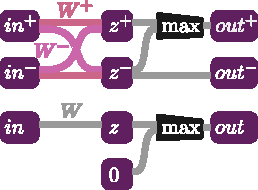
\includegraphics[width=.6\linewidth]{figures/split_streams.pdf}
    \caption{Visualization of the monotone and convex split-streams (top) in comparison to a standard ReLU layer (bottom). The negative weight matrix transitions positive input to negative preactivation and vice versa, whereas the positive part of the weight transitions from positive to positive and negative to negative.}
    \label{fig:splitstreams}
\end{figure}

\subsection{An algorithm for ReLU MLPs}\label{subsec:relu_mlp-split}

Each layer \(l \in \{1,\dots,L\}\) is replaced by a split-pair of two monotone, non-negative split-streams \(g\) and \(h\). We visualize this flow in \cref{fig:splitstreams}.
We split parameters into non-negative parts $W^{(l)} = W^{(l,+)} - W^{(l,-)}$ such that $W^{(l,+)}, \ W^{(l,-)} \geq 0$.
For more flexibility, we additionally split the input layer, replacing an input $x$ by two vectors $a^{(0,+)}$ and $a^{(0,-)}$ such that $x = a^{(0,+)} - a^{(0,-)}$. 

With this, for each \(l \in \{1,\dots,L\}\) we compute the split-stream pre-activations by
\begin{align}
      z^{(l,+)}
      &= W^{(l,+)} a^{(l-1,+)} + W^{(l,-)} a^{(l-1,-)}
      \label{eq:preact-plus} \\
      z^{(l,-)}
      &= W^{(l,-)} a^{(l-1,+)} + W^{(l,+)} a^{(l-1,-)}
      \label{eq:preact-minus}
\end{align}
By replacing the ReLU activation of the original model with a Maxout unit in the $g$-stream
one obtains, at hidden layers $l<L$, the activations $a^{(l,+)} = \max \left\{ z^{(l,+)}, z^{(l,-)} \right\}$ and $a^{(l,-)} = z^{(l,-)}$. At the final affine readout, set $a^{(L,+)}=z^{(L,+)}$ and $a^{(L,-)}=z^{(L,-)}$ without a maximum, so negative logits are preserved.
Analogously to the notation $f^{(l)}$, we denote the split-streams $g$ and $h$ restricted to the layers $l+1,\dots,L$ by $g^{(l)} : \ \RR ^ {d^{(l)}} \times \RR ^ {d^{(l)}} \longrightarrow \RR$ and $h^{(l)} : \ \RR ^ {d^{(l)}} \times \RR ^ {d^{(l)}} \longrightarrow \RR$.

We prove correctness of the split in \cref{app:fundamental}.
Indeed, the difference between the outputs of the two split-streams equals the output of the original network evaluated at the difference of their inputs.

\begin{theorem}[Correctness] \label{thm:split_correct}
    For any $x^+, x^- \in \RR^{d^{(l)}}$
    \begin{align*}
        f^{(l)} \bigl( x^+ - x^- \bigr)
            = \bigl( g^{(l)} - h^{(l)} \bigr)
                \begin{bmatrix}
                    x^+ \\
                    x^-
                \end{bmatrix},
    \end{align*}
\end{theorem}

Here, the crucial observation for the next step is that we have flexibility in representing the input $x$ as a difference $x = x^+ - x^-$.

\subsection{Numerically stabilizing the forward pass} \label{sec:forward}

As our split-pair lacks cancellation by subtraction, network activations tend to explode in deep neural networks. 
To mitigate this, we propose shifting the activations into numerically stable regimes.

By \cref{thm:split_correct},
adding the same constant shift to both \(a^{(l,+)}\) and \(a^{(l,-)}\) preserves the difference of $g^{(l)}$ and $h^{(l)}$.
For fixed shifts, the head Jacobians at shifted and unshifted split coordinates agree, as shown in \cref{app:fundamental}. Input-dependent re-centering must be detached during backpropagation to preserve these head sensitivities. Differentiating through such a shift adds a common derivative term to both heads; only their difference is guaranteed unchanged. The convexity and coordinatewise monotonicity statements concern the unshifted heads: input-dependent re-centering need not preserve these properties, even when detached for the backward computation. 
Indeed, the gradient flow is determined only by the indices, where the maximum between the split-streams preactivations are taken, and not by the preactivations actual value.
    
\paragraph{Implementation details for forward pass stabilization}
We keep activations in check by `re-centering' the pairs of
activations in the two split-streams whenever their magnitudes explode using different strategies based on thresholds, scaling, or shifting.
All intermediate computations use \texttt{torch.float64} for high numerical precision matrix multiplication.
Furthermore, we optionally cache the activations of the original model to slightly correct the activations of the split model on the fly, ensuring the \textbf{forward invariant:} $a^{(l,+)} - a^{(l,-)} = a^{(l)}$.

\subsection{Numerically stabilizing the backward pass} \label{sec:backward}

As the computation of the gradients of $g$ and $h$ involves only non-negative matrices, these quantities turn out to be very large for deep networks. 
Therefore, we subtract non-constant offsets in their iterative computation. 
While this does not result in the same numerical information as the gradient, it still captures the pattern of the activation function and preserves the relation of gradients for different inputs. 

So let $\delta^{(l,+,g)} \coloneqq \frac{\partial g^{(l)}}{\partial a^{(l,+)}}$ be the derivative of the `head' $g^{(l)}$ by the `positive part' $a^{(l,+)}$ of the split-stream activations of layer $l$, and let $\delta^{(l,-,g)}$, $\delta^{(l,+,h)}$ and $\delta^{(l,-,h)}$ be defined analogously. 
We call them \emph{local sensitivities}. 
We compute a \emph{modified gradient} by subtracting
an $\alpha^{(l)}$-multiple of the product of the absolute values of all subsequent weight matrices and then iterating this layer by layer. As we show mathematically in \cref{app:closed_formulas}, this reduces the absolute values of the local sensitivities.
We usually choose all the factors $\alpha^{(l)}$ to be the same value $\alpha$.
For $\alpha = 0.5$ the local sensitivities are just multiples of the original gradients, while for $\alpha = 0$ they resemble the actual split-pair gradients.
Hence, the most interesting regime is $0 < \alpha < 0.5$.

\paragraph{Implementation details for backward pass stabilization}
When backpropagating through ReLU and Maxpooling components, instead of using the maximum patterns of the split activations, \ie the indices, where the maximum of the split-streams preactivations are taken, we utilize the positivity patterns of the cached original network activations.
Furthermore, we cache the original network gradients and apply small corrections to ensure the \textbf{backward invariant}
    \begin{equation}
        \frac{1}{2}\left[(\delta^{(l,+,g)} - \delta^{(l,-,g)}) -
        (\delta^{(l,+,h)} - \delta^{(l,-,h)})\right]
        = \frac{\partial f^{(l)}}{\partial a^{(l)}}.
        \label{eq:backward_invariant}
    \end{equation}

\subsection{Generalization to other network components} \label{subsec:other_components}

We represent every component as a \emph{chunk module} with explicit positive/negative inputs and outputs, and we keep linear and convolutional layers and ReLU as separate chunks in order to support multiple layers without intermediate activation.

A forward/backward cache accumulates inflowing activations and gradients per chunk, and a parallel cache mirrors the original model. The latter serves both analysis (layer-wise activation/gradient error) and optional on-the-fly correction (forward and backward) and reuses the original model’s positivity patterns in place of split-pair maxima in the backward pass.
Our converter maps arbitrary PyTorch graphs (for supported layers/functions) to the split form.

We give an overview of the adaptations to split further network components into non-negative parts:
\textbf{Convolutional operations} are handled analogously to linear layers by splitting each kernel into positive and negative parts.
\textbf{Bias terms} are decomposed as \(b=b^+-b^-\) and added separately to the two streams. 
\textbf{Additive operations}, including residual connections, simply add the corresponding split activations (and distribute gradients independently).
\textbf{Average Pooling} is a positive linear operator and is therefore applied to each stream without modification.
\textbf{Batch normalization} in evaluation mode reduces to an affine map and can be treated as a special convolution; handling training-mode statistics would require the multiplicative splitting described in \cref{app:splitting_multiplicative_maxout_networks}. We also support merging Batch normalization layers with adjacent linear or convolutional Layers.
\textbf{Dropout} in evaluation mode acts as identity, while in training mode we reconstruct the original dropout mask and apply it consistently to both activations and gradients of the split-streams.
\textbf{Alternative nonlinearities} such as ELU \cite{Clevert2016_elu} or Swish \cite{Ramachandran2017_swish} can be approximated by ReLU subnetworks before applying the split procedure. A finite ReLU subnetwork is piecewise affine and therefore does not represent these smooth, non-piecewise-affine activations exactly. The split then preserves the approximating network; its discrepancy from the original activation must be evaluated separately. 
For \textbf{Max pooling}, we use the convexity-preserving identity $\max_{j\in[q]}(a_j^+ - a_j^-) = \max_{j\in[q]}\Bigl\{a_j^+ + \sum_{i\neq j} a_i^- \Bigr\} - \sum_{i} a_i^-$.

Optionally, we replace this formulation with a ``winner-takes-it-all'' (\emph{wta}) rule that forwards the locations of both split-streams, where their difference takes the maximum. This however comes at the cost of monotonicity and convexity of the split-streams.
